\section{Introduction}

Use of Deep Neural Networks, commonly referred to as
\emph{deep learning}, has spiked in recent years and has been popular
as a tool for impressive advancements in the field of 
\emph{Artificial Intelligence (AI)}.
The goal of this project was to attempt and recreate a spiking neural network that is capable of object detection, particularly classification and localization. As described, our program was built on Deep Neural Networks, spiking neurons, and convolutional network frameworks, which we find interesting and important. Despite the inability to complete the product we nonetheless met our ultimate goal; to learn more about computational neuroscience. Moreover, our attempt at an object detecting, spiking neural network provided a comprehensive learning experience for all members, regardless of prior knowledge on the subject. 

\subsection{Neural Networks}

% \subsection{Deep Neural Networks}

A Deep Neural Network, DNN, is a machine learning algorithm that tries to mimic how the brain processes information. The reason why DNNs are called deep is due to the networks having more than two hidden layers. The increased number of hidden layers enables DNNs to complete more complicated tasks compared to their shallow counterparts. However, increasing the number of hidden layers increases the training time in addition to the electrical power per epoch. 

% \subsection{Spiking Neural Network}

On the other hand, Spiking Neural Networks, SNNs, mimic both the information encoding and the process within a human brain by using spiking neurons as activation functions (\citeA{maaasSnns}). SNNs send information as a discrete series of spikes as opposed to sending continuous real values that layers of DNNs output. The SNN model is efficient because the spiking neuron only integrates its value when the membrane potential, voltage, passes the threshold which enables event-driven computation (\citeA{kim2020spiking}). However, to harness the efficiency of SNNs, they have to be trained and implemented on neuromorphic hardware.

% \section{What is Spiking in SNNs}

\subsection{Leaky Integrate and Fire}

\begin{figure}[h]
	\begin{center}
		\scalebox{0.35}{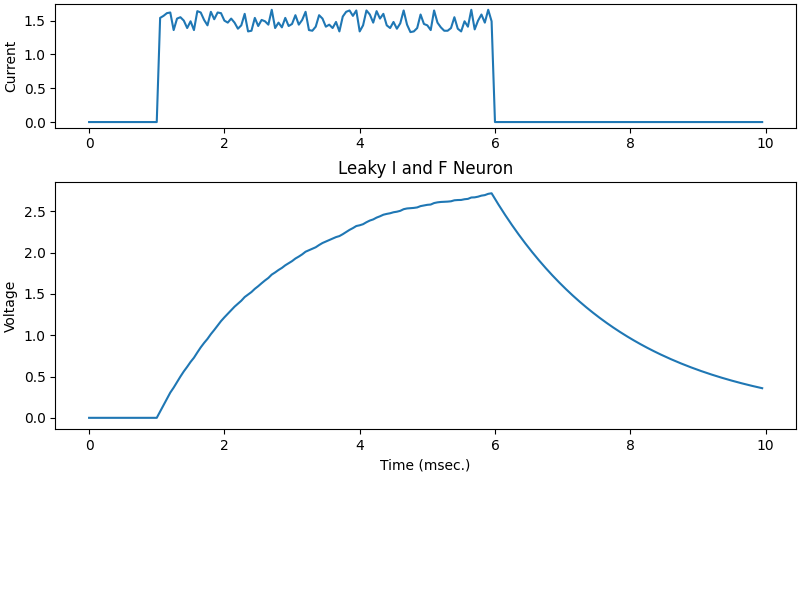
\includegraphics{LIF_plot.png}}
	
	\end{center}
	\caption{Example of a Leaky Integrate and Fire Neuron being injected with a current {i}}
\end{figure}

The Integrate and Fire model, IAF, shows how the membrane potential of a neuron reacts to an injection of current. If the membrane potential is injected with a high enough current it starts an all-or-nothing reaction resulting in a spike or action potential. The difference between the IAF model and the leaky integrate and fire model, LIF, is the existence of a reset mechanism in the LIF. Just like in the IAF model, when the LIF neuron reaches the threshold, it fires and causes a spike. However, the leaky model can reset the membrane potential's voltage by using the reset by subtraction method. The reset by subtraction method is biologically more accurate because as in real neurons, after firing, the neuron needs a higher voltage value to fire again.



% \subsection{Implementation of Membrane Potentials}

% In order to imitate behaviour of a neuron, SNNs have to keep and encode the membrane potential information. This is important, because membrane potential at the time  dictates to the neuron if it should fire, do nothing or enter refractory period. Membrane potential in SNNs can be expressed with the following equation:


% \begin{equation}
% 	V_{mem, j}^1(t) = V_{mem, j}^1(t-1) + z_j^l{t} - V_{th}\theta_j^l(t)
% \end{equation}

% \begingroup
% \fontsize{7pt}{9pt}\selectfont
% \begin{enumerate}
%     \item[] \begin{center}  $V_{mem, j}^1(t-1)$ = membrane potential at the previous time step, \end{center}
% 	\item[]  \begin{center} $z_j^l{t}$ is a sum of bias and products of weight and spikes, \end{center}
% 	\item[] \begin{center}  $V_{mem}$ = membrane voltage, \end{center}
% 	\item[] \begin{center}  $\theta_j^l(t)$ is a spike, \end{center}
% 	\item[] \begin{center}  $V_{th}$ = threshold voltage value. \end{center}
% \end{enumerate}
% \endgroup

Requirement to pass this information from layer to layer is one of the reasons why it is difficult to train Spiking Neural Networks (\citeA{kim2020spiking}). 

\section{Problems with Spiking Neural Networks}

\subsection{Loss of Information}

When a neuron in Spiking Networks is either under- or overactivated, there might occur information loss. These events happen due to the input voltage being either too large and generating spikes regardless of the value of input, or due to input voltage being too low and taking a long time to produce a spike. To solve these problems, multiple normalization methods have been invented. For example, \citeA{kim2020spiking} proposed a channel-wise data-based normalization that normalizes the weights by the maximum possible activation in a channel-wise manner as opposed to a conventional layer-wise method. 

\subsection{Non-differentiability}

The issue with the SNN is that the spike events are non-linear, discrete events, which means that the rate of change or the derivative, is zero everywhere apart from when the value of the membrane potential is equal to zero (\citeA{surrogateGradient}). Thus, the SNN model can not use standard error backpropagation.

Alleviating the issue of the SNN model’s being non-differentiability in addition to optimizing the algorithm itself required either smoothing the SNN by making it continuously differentiable, or introducing the surrogate gradient (SG) which is a “continuous relaxation of the real gradients” (\citeA{surrogateGradient}). snnTorch solves the non-differentiability issue for us by providing a custom backpropagation method that integrates surrogate gradient. 

\subsection{Biological Icarus}

Just like in the story of Icarus and his father, creators of Spiking Neural Networks are trying to get close to biologically plausible neural network models while trying to not \textit{"melt their wings"} and fail. Due to this constraint, LIF seems to be the best candidate to simulate neurons without getting into too much biological detail.

All the challenges of implementation of Spiking Neural Networks that we have mentioned before are the reason why standard Artificial Neural Networks rely on utility focused tools for achieving their goals. Indeed, introduction of more biologically plausible models are faced with problems when attempted to be implemented in code. This is the case with Leaky-Integrate-and-Fire and the reason why despite being the most biologically accurate model, the Hodgkin's and Huxley's neuron model (H-and-H) is not likely to be used in AI and development of neural networks. Moreover, if someone would try to create a neural network with H-and-H model at the heart they would probably \textit{"get too close to the sun"} and fall.